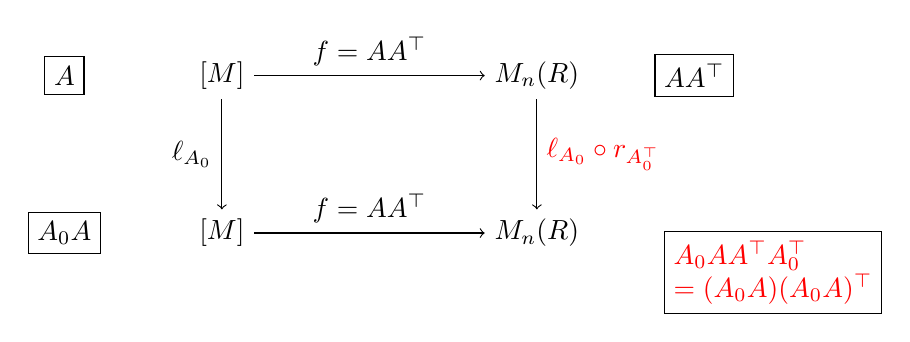
\begin{tikzpicture}
    \node (mani1) at (0, 0) {$\manifold[M]$};
    \node (real1) at (4, 0) {$M_n(\mathbb{R})$};
    \node (mani2) at (0, -2) {$\manifold[M]$};
    \node (real2) at (4, -2) {$M_n(\mathbb{R})$};
    \draw[->] (mani1) -- (real1) node[midway, above] {$f = AA ^{\top}$};
    \draw[->] (mani2) -- (real2) node[midway, above] {$f = AA ^{\top}$};
    \draw[->] (real1.south) -- (real2.north) node[midway, right, text=red] 
        {$\ell_{A_0}\circ r_{A_0 ^{\top}}$};
    \draw[->] (mani1.south) -- (mani2.north) node[midway, left] 
        {$\ell_{A_0}$};
    \node[draw] at (-2, 0) {$A$};
    \node[draw] at (-2, -2) {$A_0A$};
    \node[draw] at (6, 0) {$AA ^{\top}$};
    \node[draw, align=left, text=red] at (7, -2.5) 
    {$A_0AA ^{\top} A_0 ^{\top}$\\$=(A_0A)(A_0A) ^{\top}$};
\end{tikzpicture}